\section{Classical Response of a Single Nucleus to a Magnetic Field}

\subsection{Summary} 
\begin{enumerate}
    \item This chapter investigates a single proton's response to an external magnetic field.
    \item The magnetic moment of the spin in the presence of an external magnetic field will align with the external field as this is its equilibrium state.

    \begin{itemize}
        \item A current loop of current $I$ (and area $A$) placed in an external magnetic field $B$ will experience a differential force on the loop determined by the cross product between the differential current and the magnetic field. \\
        \begin{equation}
            d\vec{F} = I d\vec{l} \times \vec{B}
        \end{equation}

        \item The total force on this loop (or any closed loop) will be zero. This can be derived by taking the integral over the equation above. This leads to a zero change in the total momentum $p$ as: \\
        \begin{equation}
            \vec{F} = \frac{d\vec{p}}{dt}
        \end{equation}

        \item In conclusion, a current loop found at rest in a constant external magnetic field 
        will remain at rest unless external forces are applied, 
        depending on the orientation (like in Figure~\ref{fig:fig21}a). 
        Otherwise, they will experience a torque which will rotate the loop.
        \begin{figure}[H]
            \centering
            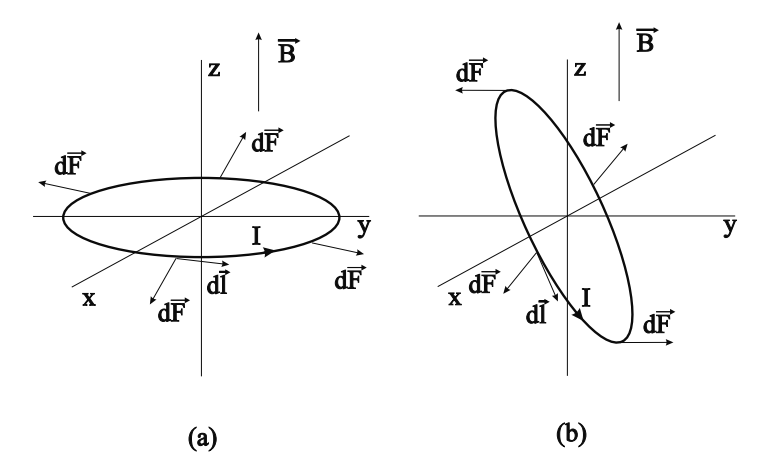
\includegraphics[width=0.6\textwidth,keepaspectratio]{fig21}
            \caption{
           Circular current loop depicted in two different orientations relative to a uniform magnetic
        field. The forces on representative differential current segments are shown (one \textit{d} is explicitly shown
        in each case). The first (a) shows the current plane perpendicular to the field where there is no
        net twist (torque); the second (b) shows the current plane at an arbitrary angle to the field where
        there is a nonzero torque. 
            }
            \label{fig:fig21}
        \end{figure}

        \item In other words, if the current loop is not at rest, then it will try to rotate itself to be at rest. Rotations can also arise from forces applied off-centre even when the sum of all differential forces is zero. Rotations are described by a force called \textbf{torque}. Each differential segment experiences a differential torque: \\
        \begin{equation}
            d\vec{N} = \vec{r} \times d\vec{F}
        \end{equation}

        \item The total sum of these differential torques is zero for non-rotating objects, and nonzero for rotating ones. This is exemplified in Figure~\ref{fig:fig21} and in Exercises \ref{fig:ex21} and \ref{fig:ex22}.

        \item For any arbitrary current distribution, the net torque has the following formula: \\
        \begin{equation} \label{eq:eq24}
            \vec{N} = \vec{\mu} \times \vec{B}
        \end{equation}
        where $\vec{\mu}$ is called the magnetic dipole moment or magnetic moment. 
        
        \item The magnetic moment vector for planar loops is given in
            terms of the current going through the loop \textit{I}, the area of the
            loop \textit{A} and the unit vector $\vec{n}$ perpendicular to the
            current loop plane \\
        \begin{equation} \label{eq:eq25}
            \vec{\mu} = I A \hat{n}
        \end{equation}
        This can be visualised in Figure~\ref{fig:fig22}.
        \begin{figure}[H]
            \centering
            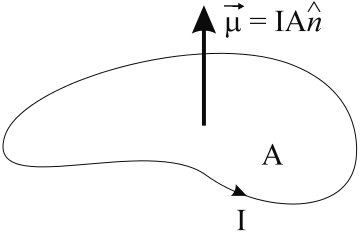
\includegraphics[width=0.4\textwidth,keepaspectratio]{fig22}
            \caption{ A loop with current I lying in a plane
            } 
            \label{fig:fig22}
        \end{figure}
        
        
        \item An example \\
            For Figure~\ref{fig:fig23a}, 
            the total torque for planar loops will depend on the current
            \textit{I} (anticlockwise), the magnetic field strength \textit{B}, the angle
            \textit{$\theta$} between the plane in which the current loop lies and the
            magnetic field and the total area of the loop. \\ 
        
        To get to this we begin with: 
        \begin{align}
            d\vec{N} = \vec{r} \times (Id\vec{l} \times \vec{B}) = Id\vec{l}(\vec{B} \cdot \vec{r}) - I \vec{B} (d\vec{l} \cdot \vec{r})
        \end{align}
        where $\vec{B}$ and the cylindrical unit vectors looking like:
        
        \begin{align}
            \vec{B} = B(cos \theta \text{ } \hat{z} + sin \theta \text{ } \hat{y}) \\
            \hat{\rho} = cos \phi \text{ } \hat{x} + sin \phi \text{ } \hat{y} \\
            \hat{\phi} = - sin \phi \text{ } \hat{x} + cos \phi \text{ } \hat{y}
        \end{align}
        
        Calculating and integrating over we arrive at:
        \begin{equation} \label{eq:eq29}
            \vec{N} = − I \pi R 2 B sin\theta \hat{x}
        \end{equation}

        \begin{figure}[H]
            \centering
            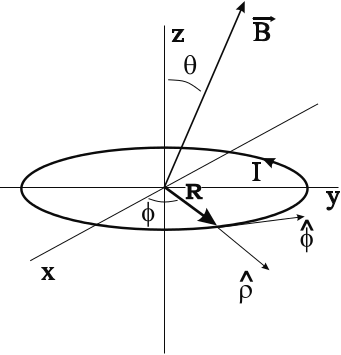
\includegraphics[width=0.4\textwidth,keepaspectratio]{fig23a}
            \caption{ A circular loop in x-y plane and the magnetic field lying in the y-z plane
            } 
            \label{fig:fig23a}
        \end{figure}

    \end{itemize}

    \item Spin has intrinsic angular momentum. Magnetic moment is proportional to it. In this case the motion is changed.
    \begin{itemize}
        \item In the picture painted so far we introduce 'spinning', or \textbf{angular momentum}.

        \begin{itemize}
            \item The change in the angular momentum of the spin will equal torque.
            \begin{equation} \label{eq:eq214}
                \frac{d\vec{J}}{dt} = \vec{N}
            \end{equation}
            
            \item This comes from (a system of many point particles with respect to some origin):
            \begin{equation} \label{eq:eq215}
                \vec{J} = \sum_i \vec{r}_i \times \vec{p}_i
            \end{equation}
            where $d\vec{p} = \vec{F} dt$
            
            \textcolor{gray}{\textbf{Sidenote}: \\
            $\vec{p}$ is linear momentum \\
            $\vec{r} \times \vec{p}$ is angular momentum    
            }
        \end{itemize}

        \item There exists a connection between intrinsic angular momentum and its moment
        \begin{itemize}
            \item The direct relationship between the magnetic moment and
            the spin angular momentum vector is found from experiment:
            \begin{equation} \label{eq:eq216}
                \vec{\mu} = \gamma \vec{J}
            \end{equation}

            where $\gamma$ is called the \textit{gyromagnetic ratio} and it depends on the particle or nucleus. For the proton nucleus it is: 
            \begin{equation} 
                \gamma = 2.675 \times 10^8 \text{rad/s/T}
            \end{equation}            
        \end{itemize}        

        \item The equation of motion of a precessing spin immersed in a static polarising magnetic field can be found using Eq~\ref{eq:eq216} and Eq~\ref{eq:eq24} in Eq~\ref{eq:eq214} (also known as a simple version of the Bloch equation):
        \begin{equation} \label{eq:eq224}
            \frac{d\vec{\mu}}{dt} = \gamma \vec{\mu} \times \vec{B}
        \end{equation}

    \end{itemize}

    \item Geometrical Representation
    \begin{multicols}{2}
    \begin{align*}
        R = \abs{\mu} \cdot sin\theta \\
        d\vec{\mu} = R \cdot \abs{d\phi} \\
        d\vec{\mu} = \abs{\vec{\mu}} \cdot sin\theta \cdot \abs{d\phi}
    \end{align*}

    \vfill
    \columnbreak

    \begin{figure}[H]
        \centering
        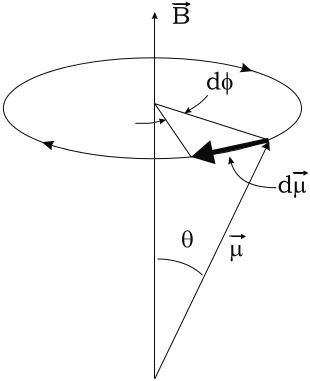
\includegraphics[width=0.3\textwidth,keepaspectratio]{fig25}
        \caption{ Clockwise precession of a proton's spin about a magnetic field.
        } 
        \label{fig:fig25}
    \end{figure}

    \end{multicols}

    \begin{equation}\label{eq:eq225}
        \abs{d\vec{\mu}} = \mu\, sin\theta\, \abs{d\phi}
    \end{equation}
    From Eq~\ref{eq:eq224}:
    \begin{equation}\label{eq:eq226}
        \abs{d\vec{\mu}} = \gamma \abs{\vec{\mu} \times \vec{B}} dt = \gamma\, \mu\, B\, sin \theta\, dt
    \end{equation}
    From Eq~\ref{eq:eq225} and ~\ref{eq:eq226} we have: $\abs{d\phi} = \gamma\, B\,dt$.\\
    Because $\omega = \abs{\frac{d\phi}{dt}}$, we get the famous Larmor precession formula:
    \begin{equation}\label{eq:eq227}
        \omega = \gamma\, B
    \end{equation}
    Also, because we have a clockwise rotation in the figure:
    \begin{equation}\label{eq:eq228}
        \frac{d\phi}{dt} = - \omega
    \end{equation}
    If the field is along the z-axis and constant in time, $\vec{B} = B_0 \hat{z}$,
    the solution for Eq~\ref{eq:eq228} is:
    \begin{equation}\label{eq:eq230}
        \phi = - \omega_0 t + \phi_0
    \end{equation}

    %%%%%%%%%%%%%%%%%%%%%%%%%%%%%%%%%%%%%%%%%%
    \item Cartesian Representation
    \begin{multicols}{2}
    \begin{align*}
        \vec{\mu_x}(t) = \vec{\mu}(t) \cdot cos(\phi_0 - \xi) \\
        \vec{\mu_x}(t) = \vec{\mu}(t) \cdot (cos \phi_0 \cdot cos \xi + sin \phi_0 \cdot sin \xi ) \\
        \vec{\mu_x}(t) = \vec{\mu}(t) \cdot cos \phi_0 \cdot cos \xi \\
        + \vec{\mu}(t) \cdot sin \phi_0 \cdot sin \xi  \\
        \vec{\mu_x}(t) = \vec{\mu}(t) \cdot \frac{\vec{\mu_x}(0)}{\vec{\mu}(0)} \cdot cos \xi \\
        + \vec{\mu}(t) \cdot  \frac{\vec{\mu_y}(0)}{\vec{\mu}(0)} \cdot sin \xi  \\
        \vec{\mu_x}(t) = \vec{\mu_x}(0) \cdot cos \xi + \vec{\mu_y}(0) \cdot sin \xi \\
    \end{align*}

    \vfill
    \columnbreak

    \begin{figure}[H]
        \centering
        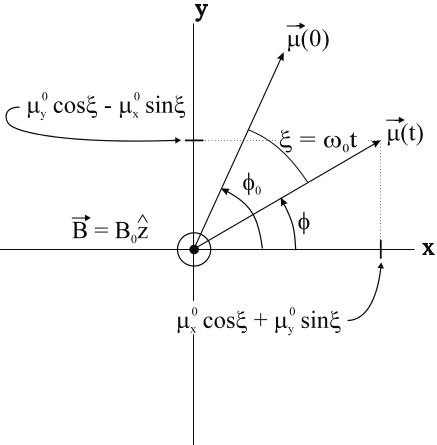
\includegraphics[width=0.4\textwidth,keepaspectratio]{fig26a}
        \caption{ } 
        \label{fig:fig26a}
    \end{figure}

    \end{multicols}

    For $\vec{B} = B_0 \hat{z}$ we have:
    \begin{equation}\label{eq:eq232}
        \vec{\mu}(t) = \vec{\mu_x}(t)\hat{x} + \vec{\mu_y}(t)\hat{y} +  \vec{\mu_z}(t)\hat{z}
    \end{equation}
    with:
    \begin{align}\label{eq:eq233}
        {\mu_x}(t) = {\mu_x}(0) \cdot cos \omega_0 t + {\mu_y}(0) \cdot sin \omega_0 t \\
        {\mu_y}(t) = {\mu_y}(0) \cdot cos \omega_0 t - {\mu_x}(0) \cdot sin \omega_0 t \\
        {\mu_z}(t) = {\mu_z}(0)
    \end{align}

    %%%%%%%%%%%%%%%%%%%%%%%%%%%%%%%%%%%%%%%%%%
    \item Matrix Representation
    \begin{equation}\label{eq:eq236}
        \vec{\mu}(t) = R_z(\omega_0t) \vec{\mu}(0)
    \end{equation}
    with:
    \begin{equation}
    R_z(\theta)=
    \begin{pmatrix}
    cos\theta & sin\theta & 0 \\
    -sin\theta & cos\theta & 0 \\
    0 & 0 & 1
    \end{pmatrix}
    \end{equation}

    %%%%%%%%%%%%%%%%%%%%%%%%%%%%%%%%%%%%%%%%%%
    \item Complex Representation and Phase
    The two degrees of freedom, ${\mu_x}$ and ${\mu_y}$, can be given in terms of the real and
    imaginary parts of:
    \begin{equation}
        {\mu_{+}}(t) = {\mu_x}(t) + i {\mu_y}(t)
    \end{equation}
    with:
    \begin{equation}
        {\mu_{+}}(t) = {\mu_{+}}(0) e^{-i\omega_0t}
    \end{equation}

    In general, the complex number ${\mu_{+}}(t)$ can be written in terms of its magnitude and phase:
    \begin{equation}
        {\mu_{+}}(t) = \abs{{\mu_{+}}(t)} e^{i\phi (t)}
    \end{equation}
    So, the complex representation can be rewritten as:
    \begin{equation}
        {\mu_{+}}(t) = \abs{{\mu_{+}}(0)} e^{i\phi_0 (t)}
    \end{equation}
    where the phase is:
    \begin{equation}
        \phi_0(t) = -\omega_0 t + \phi_0(0)
    \end{equation}

\end{enumerate}

\clearpage

%%%%%%%%%%%%%%%%%%
% \clearpage
%%%%%%%%%%%%%%%%%%%%%%%%%%%%%%%%%%%%%%%%%%
% \subsection{Magnetic Moment in the Presence of a Magnetic Field}
% \begin{itemize}
%     \item This section reviews Physics concepts such as: magnetic force, magnetic moment given by a current loop, torque due to force and torque’s relation to the magnetic moment and the magnetic field.
% \end{itemize}

% \subsubsection{Torque on a Current Loop in a Magnetic Field}
% \begin{itemize}
%     \item Placing a current loop of current $I$ (and area $A$) in an external magnetic field $B$ will create a differential force on the loop determined by the cross product between the differential current and the magnetic field. \\
%     \begin{equation}
%         d\vec{F} = I d\vec{l} \times \vec{B}
%     \end{equation}

%     \item The total force on this loop (or any closed loop) will be zero. This can be derived by taking the integral over the equation above. This leads to a zero change in the total momentum $p$ as: \\
%     \begin{equation}
%         \vec{F} = \frac{d\vec{p}}{dt}
%     \end{equation}

%     \item In conclusion, a current loop found at rest in a constant external magnetic field 
%     will remain at rest unless external forces are applied, 
%     depending on the orientation (like in Figure~\ref{fig:fig21}a). 
%     Otherwise, they will experience a torque which will rotate the loop.
%     \begin{figure}[H]
%     	\centering
%     	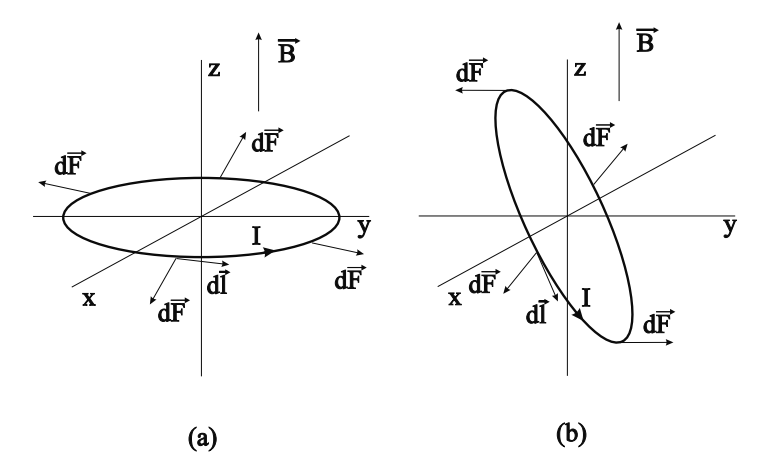
\includegraphics[width=0.6\textwidth,keepaspectratio]{fig21}
%     	\caption{
%        Circular current loop depicted in two different orientations relative to a uniform magnetic
%     field. The forces on representative differential current segments are shown (one \textit{d} is explicitly shown
%     in each case). The first (a) shows the current plane perpendicular to the field where there is no
%     net twist (torque); the second (b) shows the current plane at an arbitrary angle to the field where
%     there is a nonzero torque. 
%         }
%     	\label{fig:fig21}
%     \end{figure}

%     \item In other words, if the current loop is not at rest, then it will try to rotate itself to be at rest. Rotations can also arise from forces applied off-centre even when the sum of all differential forces is zero. Rotations are described by a force called \textbf{torque}. Each differential segment experiences a differential torque: \\
%     \begin{equation}
%         d\vec{N} = \vec{r} \times d\vec{F}
%     \end{equation}

%     \item The total sum of these differential torques is zero for non-rotating objects, and nonzero for rotating ones. This is exemplified in Figure~\ref{fig:fig21} and in Exercises \ref{fig:prbl21} and \ref{fig:prbl22}.

%     \item For any arbitrary current distribution, the net torque has the following formula: \\
%     \begin{equation} \label{eq:eq24}
%         \vec{N} = \vec{\mu} \times \vec{B}
%     \end{equation}
%     where $\vec{\mu}$ is called the magnetic dipole moment or magnetic moment. 
    
%     \item The magnetic moment vector for planar loops is given in
%         terms of the current going through the loop \textit{I}, the area of the
%         loop \textit{A} and the unit vector $\vec{n}$ perpendicular to the
%         current loop plane \\
%     \begin{equation} \label{eq:eq25}
%         \vec{\mu} = I A \hat{n}
%     \end{equation}
%     This can be visualised in Figure~\ref{fig:fig22}.
%     \begin{figure}[H]
%     	\centering
%     	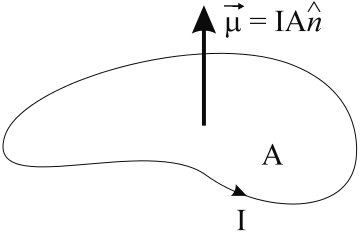
\includegraphics[width=0.4\textwidth,keepaspectratio]{fig22}
%     	\caption{ A loop with current I lying in a plane
%         } 
%     	\label{fig:fig22}
%     \end{figure}
    
    
%     \item An example: For Figure~\ref{fig:fig23a}, 
%         the total torque for planar loops will depend on the current
%         \textit{I} (anticlockwise), the magnetic field strength \textit{B}, the angle
%         \textit{$\theta$} between the plane in which the current loop lies and the
%         magnetic field and the total area of the loop. \\
%     To get to this we begin with: \\
%     $d\vec{N} = \vec{r} \times (Id\vec{l} \times \vec{B}) = Id\vec{l}(\vec{B} \cdot \vec{r}) - I \vec{B} (d\vec{l} \cdot \vec{r})$ \\
%     with $\vec{B}$ and the cylindrical unit vectors looking like:
%     \begin{align}
%         \vec{B} = B(cos \theta \text{ } \hat{z} + sin \theta \text{ } \hat{y}) \\
%         \hat{\rho} = cos \phi \text{ } \hat{x} + sin \phi \text{ } \hat{y} \\
%         \hat{\phi} = - sin \phi \text{ } \hat{x} + cos \phi \text{ } \hat{y}
%     \end{align}
%     Calculating and integrating over we get to:
%     \begin{equation} \label{eq:eq29}
%         \vec{N} = − I \pi R 2 B sin\theta \hat{x}
%     \end{equation}
%     \begin{figure}[H]
%     	\centering
%     	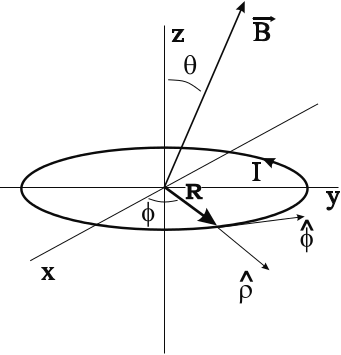
\includegraphics[width=0.4\textwidth,keepaspectratio]{fig23a}
%     	\caption{ A circular loop in x-y plane and the magnetic field lying in the y-z plane
%         } 
%     	\label{fig:fig23a}
%     \end{figure}
    
% \end{itemize}


% \subsubsection{Magnet Toy Model}
% \begin{itemize}

%     \item The picture so far can also be painted from the perspective of a dipole: 
%     2 positive and negative charges at distance $d$ one from another. 
%     In this frame we will also get a net torque of the same form as discussed before:

%     \item In terms of magnetic dipoles (see Figure~\ref{fig:fig23c}), the magnetic moment vector 
%         has the following form: \\
%         \begin{equation}  \label{eq:eq211}
%             \vec{\mu}_m = \hat{n} q_m d
%         \end{equation}
%         where $d$ is the distance between
%         the magnetic charges ($-q_m$ and $+q_m$) \\
%         The force on the magnetic charge due to a magnetic field is:\\
%         \begin{equation}  \label{eq:eq212}
%             \vec{F}_m = q_m \vec{B}
%         \end{equation}
%         Therefore, by choosing the torque reference point to lie on the
%         negative charge, the net torque will be: \\
%         $\vec{N}_m = (\hat{z}d) \times (q_m \vec{B}) $
%     \begin{figure}[H]
%     	\centering
%     	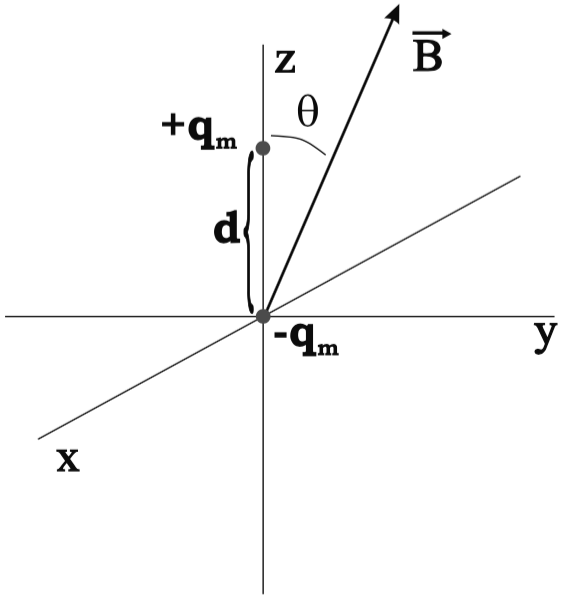
\includegraphics[width=0.4\textwidth,keepaspectratio]{fig23c}
%     	\caption{ A magnetic charge pair along the z axis } 
%     	\label{fig:fig23c}
%     \end{figure}
% \end{itemize}


% %%%%%%%%%%%%%%%%%%
% \clearpage
% %%%%%%%%%%%%%%%%%%%%%%%%%%%%%%%%%%%%%%%%%%
% \subsection{Magnetic Moment with Spin: Equation of Motion}
% \begin{itemize}
%     \item This section introduces angular momentum to the picture painted before.
% \end{itemize}

% %%%
% \subsubsection{Torque and Angular Momentum}
% \begin{itemize}
%     \item The change in the angular momentum of the spin will equal torque.
%     \begin{equation} \label{eq:eq214}
%         \frac{d\vec{J}}{dt} = \vec{N}
%     \end{equation}
    
%     \item This comes from:
%     \begin{equation} \label{eq:eq215}
%         \vec{J} = \sum_i \vec{r}_i \times \vec{p}_i
%     \end{equation}
%     where $d\vec{p} = \vec{F} dt$
    
    
%     \textcolor{gray}{\textbf{Sidenote}: \\
%     $\vec{p}$ is linear momentum \\
%     $\vec{r} \times \vec{p}$ is angular momentum    
%     }
% \end{itemize}

% %%%
% \subsubsection{Angular Momentum of the Proton}
% \begin{itemize}
%     \item 
% \end{itemize}


% %%%
% \subsubsection{Electrons and Other Elements}
% \begin{itemize}
%     \item 
% \end{itemize}

% %%%
% \subsubsection{Equation of Motion}
% \begin{itemize}
%     \item 
% \end{itemize}

% %%%%%%%%%%%%%%%%%%
% \clearpage
% %%%%%%%%%%%%%%%%%%%%%%%%%%%%%%%%%%%%%%%%%%
% \subsection{Precession Solution: Phase}
% \begin{itemize}
%     \item 
% \end{itemize}

% %%%
% \subsubsection{Precession via the Gyroscope Analogy}
% \begin{itemize}
%     \item 
% \end{itemize}

% %%%
% \subsubsection{Geometrical Representation}
% \begin{itemize}
%     \item 
% \end{itemize}

% %%%
% \subsubsection{Cartesian Representation}
% \begin{itemize}
%     \item 
% \end{itemize}

% %%%
% \subsubsection{Matrix Representation}
% \begin{itemize}
%     \item 
% \end{itemize}

% %%%
% \subsubsection{Complex Representation and Phase}
% \begin{itemize}
%     \item 
% \end{itemize}





% \clearpage
% {\huge Old Notes} \\

% In this chapter, and the next, the focus is on the basic element of the first stage, a
% single proton's response to an external field, ignoring the interactions of each proton with
% its surroundings.

% %%%%%%%%%%%%%%%%%%%%%%%%%%%%%%%%%%%%%%%%%%
% \subsection{Torque on a Current Loop in a Magnetic Field}
% When an external field $\vec{B}$ is turned on, a circular loop of current I and area A will feel a differential force on each of its differential segments d$\vec{l}$ given by the basic Lorentz force law:




% The total force on the circular loop, and indeed on any closed loop, due to a uniform
% (constant over space) external magnetic field is zero. 
% Zero total force means zero change in the total momentum $\vec{p}$, from Newton's law:


% Therefore, a current loop initially at rest in a spatially constant magnetic field stays at rest.
% But, it can be rotated by the field. The vector quantity used to describe the rotation of an object is torque:


% The formula for the net torque on any current distribution, which is exact in a 
% constant magnetic field, is given in terms of the \textit{magnetic dipole moment} 
% or simply \textit{magnetic moment} $\mu$:


% The magnetic moment vector for planar loops is given by (and see Figure~\ref{fig:fig22})



% For Figure~\ref{fig:fig23a} the differential torque on $d\vec{l}$ can be written quite generally as:






% \textbf{Takeaway:} A magnetic moment, such as that corresponding to a current loop or a bar magnet, 
% will try to line up along the direction of an external magnetic field.

% %%%%%%%%%%%%%%%%%%%%%%%%%%%%%%%%%%%%%%%%%%
% \subsection{Magnetic Moment with Spin: Equation of Motion}
% Nonzero total torque on a system implies that the system’s total angular momentum J must
% change according to:
% \begin{equation} \label{eq:eq214}
%     \frac{d\vec{J}}{dt} = \vec{N}
% \end{equation}

% The direct relationship between the magnetic moment and
% the spin angular momentum vector is found from experiment:
% \begin{equation} \label{eq:eq216}
%     \vec{\mu} = \gamma \vec{J}
% \end{equation}

% Using Eq~\ref{eq:eq216} and Eq~\ref{eq:eq24} in Eq~\ref{eq:eq214}, we get 
% the fundamental equation of motion (a simple version of the Bloch equation):
% \begin{equation} \label{eq:eq224}
%     \frac{d\vec{\mu}}{dt} = \gamma \vec{\mu} \times \vec{B}
% \end{equation}

% %%%%%%%%%%%%%%%%%%%%%%%%%%%%%%%%%%%%%%%%%%
% \subsection{Geometrical Representation}
% \begin{multicols}{2}
% \begin{align*}
%     R = \abs{\mu} \cdot sin\theta \\
%     d\vec{\mu} = R \cdot \abs{d\phi} \\
%     d\vec{\mu} = \abs{\vec{\mu}} \cdot sin\theta \cdot \abs{d\phi}
% \end{align*}

% \vfill
% \columnbreak

% \begin{figure}[H]
% 	\centering
% 	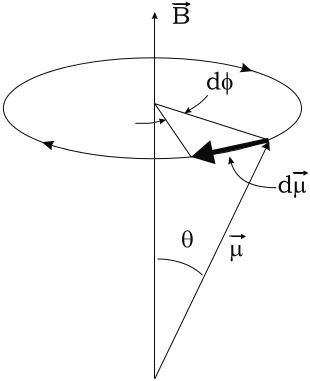
\includegraphics[width=0.3\textwidth,keepaspectratio]{fig25}
% 	\caption{ Clockwise precession of a proton's spin about a magnetic field.
%     } 
% 	\label{fig:fig25}
% \end{figure}

% \end{multicols}

% %\clearpage

% \begin{equation}\label{eq:eq225}
%     \abs{d\vec{\mu}} = \mu\, sin\theta\, \abs{d\phi}
% \end{equation}
% From Eq~\ref{eq:eq224}:
% \begin{equation}\label{eq:eq226}
%     \abs{d\vec{\mu}} = \gamma \abs{\vec{\mu} \times \vec{B}} dt = \gamma\, \mu\, B\, sin \theta\, dt
% \end{equation}
% From Eq~\ref{eq:eq225} and ~\ref{eq:eq226} we have: $\abs{d\phi} = \gamma\, B\,dt$.\\
% Because $\omega = \abs{\frac{d\phi}{dt}}$, we get the famous Larmor precession formula:
% \begin{equation}\label{eq:eq227}
%     \omega = \gamma\, B
% \end{equation}
% Also, because we have a clockwise rotation in the figure:
% \begin{equation}\label{eq:eq228}
%     \frac{d\phi}{dt} = - \omega
% \end{equation}
% If the field is along the z-axis and constant in time, $\vec{B} = B_0 \hat{z}$,
% the solution for Eq~\ref{eq:eq228} is:
% \begin{equation}\label{eq:eq230}
%     \phi = - \omega_0 t + \phi_0
% \end{equation}

% %%%%%%%%%%%%%%%%%%%%%%%%%%%%%%%%%%%%%%%%%%
% \subsection{Cartesian Representation}
% \begin{multicols}{2}
% \begin{align*}
%     \vec{\mu_x}(t) = \vec{\mu}(t) \cdot cos(\phi_0 - \xi) \\
%     \vec{\mu_x}(t) = \vec{\mu}(t) \cdot (cos \phi_0 \cdot cos \xi + sin \phi_0 \cdot sin \xi ) \\
%     \vec{\mu_x}(t) = \vec{\mu}(t) \cdot cos \phi_0 \cdot cos \xi \\
%     + \vec{\mu}(t) \cdot sin \phi_0 \cdot sin \xi  \\
%     \vec{\mu_x}(t) = \vec{\mu}(t) \cdot \frac{\vec{\mu_x}(0)}{\vec{\mu}(0)} \cdot cos \xi \\
%     + \vec{\mu}(t) \cdot  \frac{\vec{\mu_y}(0)}{\vec{\mu}(0)} \cdot sin \xi  \\
%     \vec{\mu_x}(t) = \vec{\mu_x}(0) \cdot cos \xi + \vec{\mu_y}(0) \cdot sin \xi \\
% \end{align*}

% \vfill
% \columnbreak

% \begin{figure}[H]
% 	\centering
% 	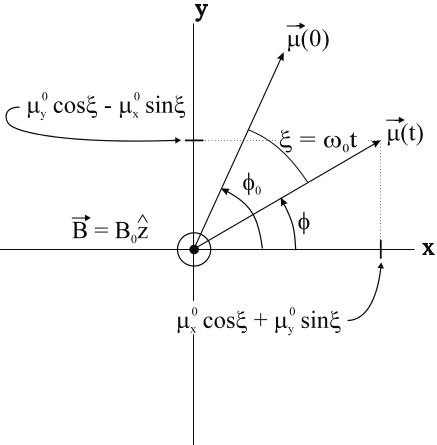
\includegraphics[width=0.4\textwidth,keepaspectratio]{fig26a}
% 	\caption{ } 
% 	\label{fig:fig26a}
% \end{figure}

% \end{multicols}

% For $\vec{B} = B_0 \hat{z}$ we have:
% \begin{equation}\label{eq:eq232}
%     \vec{\mu}(t) = \vec{\mu_x}(t)\hat{x} + \vec{\mu_y}(t)\hat{y} +  \vec{\mu_z}(t)\hat{z}
% \end{equation}
% with:
% \begin{align}\label{eq:eq233}
%     {\mu_x}(t) = {\mu_x}(0) \cdot cos \omega_0 t + {\mu_y}(0) \cdot sin \omega_0 t \\
%     {\mu_y}(t) = {\mu_y}(0) \cdot cos \omega_0 t - {\mu_x}(0) \cdot sin \omega_0 t \\
%     {\mu_z}(t) = {\mu_z}(0)
% \end{align}

% %%%%%%%%%%%%%%%%%%%%%%%%%%%%%%%%%%%%%%%%%%
% \subsection{Matrix Representation}
% \begin{equation}\label{eq:eq236}
%     \vec{\mu}(t) = R_z(\omega_0t) \vec{\mu}(0)
% \end{equation}
% with:
% \begin{equation}
% R_z(\theta)=
% \begin{pmatrix}
% cos\theta & sin\theta & 0 \\
% -sin\theta & cos\theta & 0 \\
% 0 & 0 & 1
% \end{pmatrix}
% \end{equation}

% %%%%%%%%%%%%%%%%%%%%%%%%%%%%%%%%%%%%%%%%%%
% \subsection{Complex Representation and Phase}
% The two degrees of freedom, ${\mu_x}$ and ${\mu_y}$, can be given in terms of the real and
% imaginary parts of:
% \begin{equation}
%     {\mu_{+}}(t) = {\mu_x}(t) + i {\mu_y}(t)
% \end{equation}
% with:
% \begin{equation}
%     {\mu_{+}}(t) = {\mu_{+}}(0) e^{-i\omega_0t}
% \end{equation}

% In general, the complex number ${\mu_{+}}(t)$ can be written in terms of its magnitude and phase:
% \begin{equation}
%     {\mu_{+}}(t) = \abs{{\mu_{+}}(t)} e^{i\phi (t)}
% \end{equation}
% So, the complex representation can be rewritten as:
% \begin{equation}
%     {\mu_{+}}(t) = \abs{{\mu_{+}}(0)} e^{i\phi_0 (t)}
% \end{equation}
% where the phase is:
% \begin{equation}
%     \phi_0(t) = -\omega_0 t + \phi_0(0)
% \end{equation}





